\documentclass[brazil,hardcopy,openany,a5paper]{ufscthesis}
\usepackage[brazil]{babel}
\usepackage{amsfonts, amsmath, amsthm, amsbsy,amssymb,bm,mathtools} % For math fonts, symbols and environments %
\usepackage{graphicx} 		% Required for including images
\usepackage{transparent}	% may be required for inkscape pdf figures (http://bit.ly/18i5Oga)
\usepackage{listings}
\usepackage[abnt-emphasize=bf]{abntex2cite}
\usepackage{caption}
\usepackage{multirow}
\usepackage{lscape}
\usepackage[T1]{fontenc}
\sloppy
\usepackage{siunitx}
\usepackage{nameref}
\usepackage{float}

\newcommand{\source}[1]{\small \caption*{Fonte: {#1}} } % Criar fonte embaixo da figura

\newsubfloat{figure}		% Allow subfloats in figure environment (http://bit.ly/1C20NAj)
\graphicspath{{figures/}} 	% Location of the graphics files

\usepackage{siunitx} % units package
\let\DeclareUSUnit\DeclareSIUnit
\let\US\SI
\let\us\si
\DeclareUSUnit\inch{in}
\sisetup{detect-all}  %it may be necessary to load it after loading the font package

\citebrackets[]

%----------------------------------------------------------------------
% Comandos criados pelo usuário
\newcommand{\afazer}[1]{{\color{red}{#1}}} % Para destacar uma parte a ser trabalhada
\DeclareMathOperator*{\argmin}{\arg\!\min}
\DeclareMathOperator*{\argmax}{\arg\!\max}

%----------------------------------------------------------------------
% Identificadores do trabalho
% Usados para preencher os elementos pré-textuais
\instituicao[a]{Universidade Federal de Santa Catarina} % Opcional
\departamento[a]{Biblioteca Universitária}
\programa[o]{Programa de Pós-Graduação em Engenharia Civil} 
\curso{Engenharia de Engenharia Civil}
\documento[a]{Dissertação} % [o] para dissertação e trabalho de conclusão de curso [a] para tese
\grau{Mestre} % doutor, mestre, engenheiro, etc.
\titulo{PREDIÇÃO DE CONFORTO TÉRMICO EM ESCRITÓRIOS VENTILADOS NATURALMENTE POR MEIO DE REDES NEURAIS ARTIFICIAIS}
\subtitulo{} % Opcional
\autor{Marcelo Salles Olinger}
\local{Florianópolis} % Opcional (Florianópolis é o padrão)
\data{28}{Fevereiro}{2019}
\orientador[Universidade Federal de Santa Catarina]{Profa. Ana Paula Melo, Dra.}

\begin{document}
	
	\frontmatter
	\folhaderosto[]%pre/Ficha_Catalografica.pdf]
	
	\mainmatter

	\chapter{Introdução}
	\label{chapter:introducao}
	
	De acordo com a Agência Internacional de Energia (IEA) \cite{IEA2018}, o consumo de energia elétrica global destinado ao resfriamento de edificações em 2016 foi de 2.020 TWh/ano, correspondendo a quase um quinto do consumo total no setor. A demanda por energia destinada ao resfriamento de ar em edificações mais que triplicou do ano de 1990 a 2016 e, se não houver mudanças no cenário atual, estima-se que essa demanda mais que triplicará até o ano de 2050, representando 37\% do aumento no consumo de eletricidade em edificações. Isso corresponderá a 11,5\% do consumo de energia total em edificações comerciais. O relatório da IEA mostra que esse cenário de aumento na demanda de energia é ainda mais impactante em países em desenvolvimento de clima quente. Apenas 8\% das 2,8 bilhões de pessoas que vivem nas partes mais quentes do mundo hoje possui condicionamento de ar para resfriamento. No caso Brasil, a parcela do resfriamento de ar nas cargas de pico das redes elétricas em 2016 correspondia a 7,6\% do total. A estimativa considerando-se o crescimento econômico e populacional, é de que essa parcela possa representar 30,8\% da carga de pico até o ano de 2050, se nenhuma medida for tomada para a mitigação do problema. O aumento na demanda por energia é fundamental para o desenvolvimento econômico, porém pode causar grandes impactos ambientais, como poluição, alterações climáticas e esgotamento dos recursos naturais. Para garantir a melhora na qualidade de vida de forma sustentável, busca-se políticas de incentivo à eficiência energética. No Brasil, desde 2009 o INMETRO possui um programa de etiquetagem de edificações voltado para padrões de eficiência energética de edificações \cite{BRASIL2009}.
	
	A redução dos impactos ambientais relacionados ao resfriamento de edificações pode ser alcançada através da geração de energia proveniente de fontes renováveis, do desenvolvimento de equipamentos com maior eficiência energética, ou pela busca de soluções passivas. O resfriamento passivo é um conjunto de técnicas sustentáveis para resfriar edifícios por meios naturais \cite{Samani2016}. Consiste em qualquer sistema que busca minimizar, ou eliminar se possível, o uso de sistemas de condicionamento de ar, com o objetivo de reduzir as altas temperaturas internas e o consumo de energia para resfriamento, proporcionando conforto térmico para os ocupantes.
	
	Uma das técnicas de resfriamento passivo é a ventilação natural (VN). A VN como estratégia para resfriamento de edificações é um dos componentes fundamentais no projeto de edifícios energeticamente eficientes. Técnicas de VN são encontradas ao longo de toda a história na arquitetura vernacular  \cite{Pesic2018}, e hoje vêm sendo atualizadas de acordo com novos estudos no campo de conforto térmico e projetos sustentáveis de edificações. Além de assegurar a qualidade do ar, a VN promove o resfriamento da edificação, proporcionando conforto térmico aos usuários quando as condições do clima externo são favoráveis \cite{Yao2009}.
	
	Para que o conforto térmico dos usuários seja garantido sem um consumo significativo de energia, é importante entender como ocorrem as variações térmicas em um edifício antes de construí-lo. Análises durante os estágios iniciais de projeto de uma edificação com VN podem apontar decisões fundamentais para o desempenho térmico. No estágio inicial de projeto, o potencial de otimização é maior e nesta etapa qualquer estimativa da influência dos ocupantes no conforto e desempenho energético da edificação pode refletir nas tomadas de decisão \cite{Belleri2014, Roetzel2014}.
	
	Atualmente, a forma mais avançada de predição do desempenho energético de edificações é a simulação computacional. No entanto, esse processo pode exigir o conhecimento técnico de um especialista. Simulações energéticas dinâmicas requerem modelos detalhados e enfrentam diversos problemas, associados principalmente a informações necessárias para dados de entrada do modelo processado \cite{Corgnati2013}. Uma alternativa para contornar essas questões, facilitando o uso dessa ferramenta por arquitetos e projetistas, é o desenvolvimento de metamodelos. Metamodelos são modelos gerados a partir de simulações computacionais, através dos quais é possível se obter resultados próximos aos de simulações de desempenho energético complexas.
	
	Metamodelos para eficiência energética de edificações podem ser desenvolvidos a partir de diferentes métodos \cite{Ostergard2018}. A solução mais apropriada depende do contexto e propósitos de cada aplicação.
	\citeauthoronline{Versage2015} \cite{Versage2015} foi capaz de estimar as cargas térmicas de edificações comerciais através de diferentes métodos de metamodelagem.
	\citeauthoronline{Melo2016} \cite{Melo2016} desenvolveram um modelo de redes neurais artificiais (ANN) para estimar graus hora de resfriamento e cargas térmicas de aquecimento e resfriamento em edificações residenciais.
	O desenvolvimento de um metamodelo de máquina de vetores de suporte capaz de estimar conforto térmico em edificações comerciais foi proposto por \citeauthoronline{Rackes2016} \cite{Rackes2016}. Voltado principalmente a tipologias de escolas, o metamodelo estima a fração de horas em desconforto por calor dos ocupantes ao longo do ano.
	
	A VN em edificações apresenta comportamentos complexos e a avaliação do seu potencial de resfriamento faz-se necessária desde a fase inicial de projeto. Possibilitar esse tipo de análise de forma simples e rápida pode ser fundamental nas tomadas de decisão em projetos de edificações e na aplicação de políticas públicas voltadas à eficiência energética. Por meio de ferramentas de aprendizagem automática, surge a oportunidade de se desenvolver metamodelos capazes de obter resultados de conforto térmico em edificações.
	
	\section{Objetivos}
		\subsection{Objetivo geral}

	O objetivo deste estudo é desenvolver um metamodelo capaz de estimar o conforto térmico em edifícios de escritórios ventilados naturalmente.
	
		\subsection{Objetivos específicos}
	
	Dentre os objetivos específicos deste trabalho, destacam-se:

		\begin{itemize}
			\item identificar o universo de possíveis características encontradas em edifícios de escritórios ventilados naturalmente em São Paulo;
			\item definir as variáveis com maior e menor influência no desempenho térmico dos edifícios ventilados naturalmente;
			\item desenvolver um modelo de simulação termoenergética com apenas uma zona térmica representando uma sala de escritório, capaz de representar as trocas térmicas com um edifício. % MELHORAR!!!
		\end{itemize}
	
	\chapter{Metodologia}
		\label{chapter:metodologia}

		\section{Definição dos parâmetros de entrada e saída}
		
		\subsection{Parâmetros de entrada}
		
		A princípio, a definição dos parâmetros adotados para gerar a base de dados de simulações para o desenvolvimento do metamodelo foram obtidos a partir do banco de dados com 153 edificações de escritórios com ventilação natural (VN) disponibilizado por \citeauthoronline{Pereira2018} \cite{Pereira2018}.  		
		Dentre as informações  disponíveis no banco de dados, obtém-se:
		
		\begin{itemize}
			\item orientação solar do edifício;
			\item número de pavimentos;
			\item forma dos pavimentos e das salas;
			\item áreas dos pavimentos e das salas;
			\item altura do pé-direito das salas;
			\item relações entre as dimensões dos pavimentos e entre as dimensões das salas;
			\item absortância das paredes externas; % 0.2 - 0.8
			\item espessura das paredes externas;
			\item cor da cobertura;
			\item tipo de vidro nas janelas;
			\item tipo de esquadria;
			\item fator de abertura das janelas;
			\item altura das esquadrias;
			\item percentual de abertura na fachada (PAF);  % 0 - 80
			\item tipo de sombreamento;  % 0 - 80
			\item tipo de estratégia de VN (unilateral ou cruzada).
		\end{itemize} 
		
		Os valores desses parâmetros foram observadas através de suas distribuições de ocorrência. Desta forma definiu-se os limites mínimos e máximos para o desenvolvimento das simulações termoenergéticas, com parâmetros variando de acordo com o que comumente se encontra em edifícios reais. Como as edificações do banco de dados localizam-se na cidade de São Paulo, esse foi o clima para qual o metamodelo foi desenvolvido.
		
		Certas informações não estão disponibilizadas pelo banco de dados analisado, como as relacionadas às propriedades termofísicas dos materiais da envoltória, às densidades de potência de iluminação e equipamentos, e aos padrões e taxas de ocupação. Esses valores foram definidos a partir da \citeauthoronline{INIC} \cite{INIC}. %, através da Tabela 4.1, da Tabela A.1 do anexo A e da Tabela B.I.1 do anexo B.  % Hora início e fim: 8 - 18,  INI-C
		
		Os parâmetros apresentados na Tabela \ref{table:paramconst} mantiveram-se com valores constantes no desenvolvimento do trabalho. Esses valores foram escolhidos a partir do que é apresentado na \citeauthoronline{INIC} \cite{INIC} para a modelagem das edificações nas condições de referência. A cobertura tem suas propriedades termofísicas baseadas na consideração de uma laje de concreto de 10cm e telha de fibrocimento, separadas por uma câmara de ar. O padrão de ocupação foi definido de acordo com o que é estabelecido para a análise de conforto térmico em edificações de escritórios pelo método simplificado, considerando-se apenas dias de semana. As propriedades termofísicas do piso em contato com solo e da laje entre pavimentos não são mencionadas na INI-C, portanto foi considerado, para ambos os casos, uma laje de concreto de 12cm com uma camada de piso cerâmico.
		
		\begin{table}[h]
			\centering
			\caption{Parâmetros com valores constantes.}
			\label{table:paramconst}
			\begin{tabular}{|l |r |}
				\hline
				\textbf{Parâmetro} & \textbf{Valor} \\
				\hline
				Capacidade térmica da cobertura & 233 kJ/m$^2$K \\
				\hline
				Transmitância da cobertura & 2,06 W/m$^2$K \\
				\hline
				Capacidade térmica do piso / laje & 306 kJ/m$^2$K \\
				\hline
				Transmitância do piso / laje & 4,30 W/m$^2$K \\
				\hline
				Transmitância do vidro & 5,7 W/m$^2$K \\
				\hline 
				Densidade de potência de iluminação & 14 W/m$^2$ \\
				\hline 
				Densidade de potência de equipamentos & 97 W/pessoa \\
				\hline 
				Hora de início de ocupação & 8 horas \\
				\hline 
				Hora final de ocupação & 18 horas \\
				\hline 
			\end{tabular}
%			\begin{flushleft}
%				Fonte: \citeauthoronline{INIC} \cite{INIC}, adaptado pelo autor.
%			\end{flushleft}				
		\end{table}
		
		A Tabela \ref{table:paraminic} apresenta os parâmetros que tiveram seus limites mínimos e máximos baseados nos limites apresentados na \citeauthoronline{INIC} \cite{INIC} para a aplicação do método simplificado, tanto para edificações condicionadas artificialmente, quanto para edificações naturalmente ventiladas ou híbridas.
		A única excessão é a taxa de ocupação, que é sempre considerada com o valor fixo de 0,10 pessoas/m$^2$ na \citeauthoronline{INIC}. No entanto, sabendo-se da influência que a carga térmica proveniente dos ocupantes e equipamentos elétricos pode ter nas temperaturas das zonas térmicas, optou-se por variar a taxa de ocupação entre a metade e o dobro do que é definido pela instrução normativa. A densidade de potência dos equipamentos varia de acordo com a taxa de ocupação, como apresentado previamente na Tabela \ref{table:paramconst}.
		
		\begin{table}[h]
			\centering
			\caption{Limites mínimos e máximos de valores dos parâmetros variáveis não disponíveis no banco de dados.}
			\label{table:paraminic}
			\begin{tabular}{|l |r |}
				\hline
				\textbf{Parâmetro} & \textbf{Faixa de valores} \\
				\hline
				Capacidade térmica da parede & 0,22 - 450 [kJ/m$^2$K] \\
				\hline
				Transmitância da parede & 0,50 4,40 [W/m$^2$K] \\
				\hline
				Fator solar do vidro & 0,20 - 0,87 [-] \\
				\hline 
				Ângulo horizontal de sombreamento & 0 - 80 [$^{\circ}$] \\
				\hline 
				Taxa de ocupação & 0,05 - 0,20 [pessoas/m$^2$] \\
				\hline 
			\end{tabular}
%			\begin{flushleft}
%				Fonte: \citeauthoronline{INIC} \cite{INIC}, adaptado pelo autor.
%			\end{flushleft}				
		\end{table}
	
		\subsection{Parâmetro de saída}
		
		A variável de saída do metamodelo desenvolvido é a fração de horas de desconforto por calor (EHF). Neste trabalho, o indicador escolhido para o limite superior da temperatura é estabelecido pelo método de conforto adaptativo da \citeauthoronline{ASHRAEStandard552017} \cite{ASHRAEStandard552017}, para 80\% de satisfação entre os ocupantes. O desconforto por frio não foi considerado.

		Durante as simulações, para cada \textit{timestep} com ocupação na sala, foi calculado se a temperatura operativa da zona térmica ultrapassou o limite superior determinado pelo método adaptativo da \citeauthoronline{ASHRAEStandard552017} \cite{ASHRAEStandard552017}. Ao fim de cada simulação, a fração de horas de desconforto foi obtida para cada zona térmica modelada, de acordo com a Equação \ref{eq:EHF}:
		
		\begin{equation}
		\label{eq:EHF}
		EHF = \frac{timesteps_{sup}}{timesteps_{ocup}}
		\end{equation}
		
		Onde:
		
		$EHF$ é igual a fração de horas de desconforto por calor na zona térmica;
		
		$timesteps_{sup}$ é igual ao número de \textit{timesteps} em que há ocupação na zona térmica e a temperatura operativa ultrapassa o limite superior determinado pelo método adaptativo;
		
		$timesteps_{ocup}$ é igual ao número de \textit{timesteps} em que há ocupação na zona térmica.
		\\
		
		Para avaliar o potencial do uso de ventiladores, o movimento do ar foi considerada para o desenvolvimento metamodelo.
		A \citeauthoronline{ASHRAEStandard552017} \cite{ASHRAEStandard552017} considera um aumento no limite superior da faixa de conforto térmico de acordo com a velocidade do ar.
		O aumento de aceitabilidade da temperatura operativa foi considerado para os três valores de velocidade do ar apresentados na Tabela \ref{table:var}, além da possibilidade se assumir o valor de velocidade do ar igual a zero, caso o uso de ventilador não tenha sido considerado.
		
		\begin{table}[h]
			\centering
			\caption{Aumento no limite superior da faixa de conforto em relação à velocidade do ar.}
			\label{table:var}
			\begin{tabular}{|c |c |}
				\hline
				\textbf{Velocidade média do ar} & \textbf{Temperatura} \\
				\hline
				0,6 m/s & 1,2 K \\
				\hline
				0,9 m/s & 1,8 K \\
				\hline
				1,2 m/s & 2,2 K \\
				\hline 
			\end{tabular}
			\begin{flushleft}
				Fonte:  \citeauthoronline{ASHRAEStandard552017} \cite{ASHRAEStandard552017}.
			\end{flushleft}				
		\end{table}
	
		Como o modelo de ventilação natural do programa EnergyPlus não calcula a velocidade do ar dentro das zonas, a consideração foi aplicada após as simulações, no momento da avaliação do conforto em cada \textit{timestep}. A consideração da velocidade do ar foi realizada de acordo com a Equação \ref{eq:Tsup}.
		
		\begin{equation}
		\label{eq:Tsup}
		T_{sup} = T_{sup,0} + T_{v_{ar}}
		\end{equation}
		
		Onde:
		
		$T_{sup}$ é igual à temperatura limite superior na faixa de conforto, considerando-se a velocidade do ar;
		
		$T_{sup,0}$ é igual à temperatura limite superior na faixa de conforto definida pelo método adaptativo, sem considerar a velocidade do ar;
		
		$T_{v_{ar}}$ é igual à margem extra de temperatura permitida pela consideração da velocidade do ar.
		\\
		
		\section{Simulação termoenergética}
		
		\subsection{Simulações de referência}
		
		Sabendo-se que o metamodelo prediz o conforto térmico baseado no método adaptativo da \citeauthoronline{ASHRAEStandard552017} \cite{ASHRAEStandard552017}, o principal dado de saída a se obter nas simulações foi a temperatura operativa da zona térmica, assim como a temperatura do ar externo. Portanto, todo o desenvolvimento das simulações termoenergéticas do trabalho foi voltado para que se obtivesse, com boa precisão, a temperatura operativa das zonas térmicas e, posteriormente, a sua relação com a temperatura do ar externo, chegando-se ao indicador de conforto térmico.
		
%		A Tabela \ref{table:parametros} apresenta os parâmetros que serão considerados no desenvolvimento dos modelos, com suas faixas de valores admitidos.	
%		
%		\begin{table}[h]
%			\centering
%			\caption{Parâmetros considerados e variação nos valores.}
%			\label{table:parametros}
%			\begin{tabular}{|l |r |}
%				\hline
%				\textbf{Parâmetro} & \textbf{Valores admitidos} \\
%				\hline
%				Área da zona & 12 - 100 [m$^2$] \\
%				\hline
%				Razão entre largura e profundidade & 0,5 - 2,0 [-] \\
%				\hline
%				Altura do pavimento & 0 - 30 [m] \\
%				\hline 
%				Azimute do eixo principal & 0 - 359 [$^{\circ}$] \\
%				\hline 
%				Pé-direito & 2,4 - 3,2 [m] \\
%				\hline 
%				Percentual de abertura da fachada & 0,1 - 0,6 [-] \\
%				\hline 
%				Fator de abertura da janela & 0,1 - 1 [-] \\
%				\hline 
%				Fator solar do vidro & 0,30 - 0,87 [-] \\
%				\hline 
%				Transmitância da parede & 0,5 - 4,7 [W/m$^2$K] \\
%				\hline 
%				Capacidade térmica da parede & 20 - 400 [kJ/m$^2$K] \\
%				\hline 
%				Absortância da parede & 0,2 - 0,9 [-] \\
%				\hline 
%				Sombreamento & 0 - 50 [$^{\circ}$] \\
%				\hline 
%				Densidade de ocupação & 0,05 - 0,50 [pessoas/m$^2$] \\
%				\hline 
%			\end{tabular}
%			\begin{flushleft}
%				Fonte: o autor.
%			\end{flushleft}				
%		\end{table}

		As simulações foram realizadas através do programa de simulação computacional EnergyPlus 8.9 \cite{EnergyPlus2018} e os modelos simulados foram obtidos a partir da parametrização de uma tipologia base, que permite a variação de diferentes parâmetros.  % variados pelo método de amostragem do hipercubo latino (HCL).
		Inicialmente, cada simulação representou um pavimento de uma edificação com seis salas de escritórios, onde cada sala representava uma zona térmica (Figura \ref{fig:croqui}).
		O solo foi modelado pelos objetos do \textit{Ground Domain}, nos casos onde o contato com solo foi considerado. As superfícies superiores e inferiores consideradas ajacentes a outros pavimentos do edifício foram modeladas como adiabáticas.
		
		\begin{figure}[h]
			\centering
			\caption{Croqui da tipologia base}
			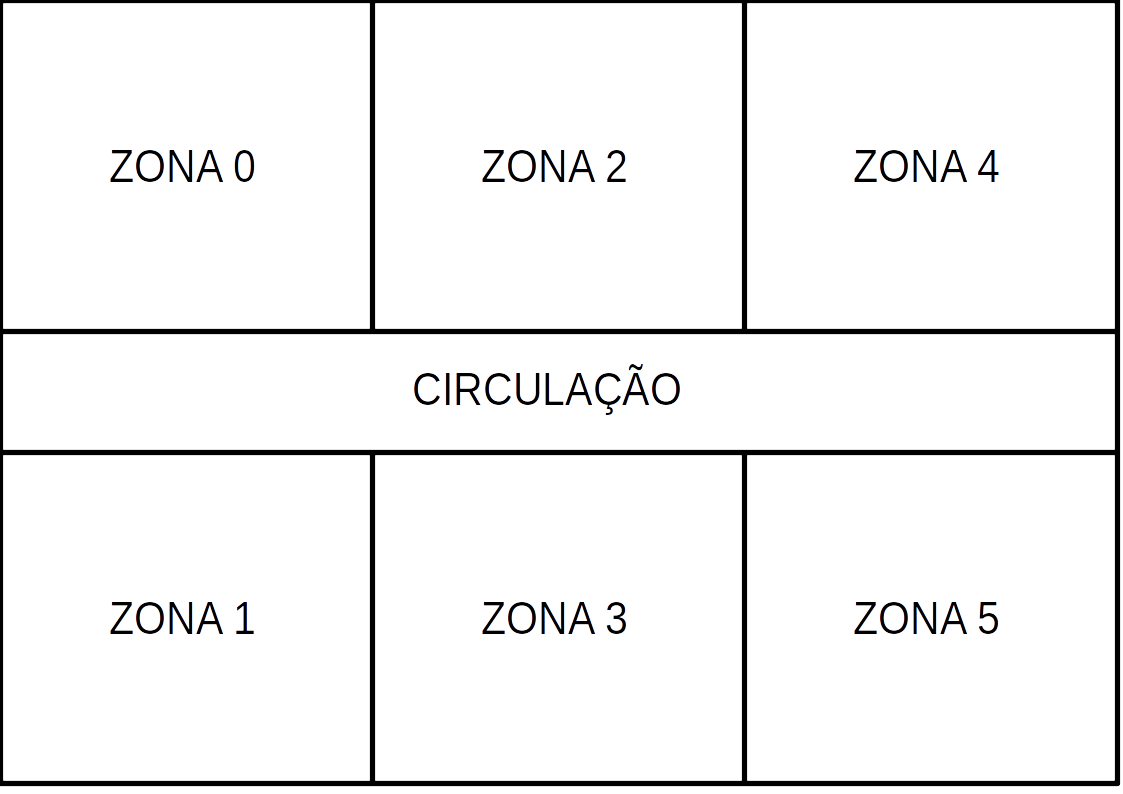
\includegraphics[width=1\linewidth]{img/croqui.png}
			\label{fig:croqui}
%			\begin{flushleft}
%				Fonte: o autor.
%			\end{flushleft}
		\end{figure}
		
		
		A partir da tipologia base, foi possível definir diferentes proporções geométricas, levando-se em consideração a largura, profundidade, altura da edificação e o pé-direito. Também foram parametrizadas a altura do pavimento e a orientação solar da edificação.
		Devido a limitações na obtenção dos coeficientes de pressão (Cp) para as faces externas da edificação, as edificações foram modeladas com pavimentos de forma retangular.
		
		A parametrização nas propriedades termofísicas das paredes e vidros permitiu a consideração de diferentes materiais construtivos, possibilitando a descrição de uma quantidade significativa do universo de casos aplicáveis às edificações de escritórios consideradas. %Foram parametrizadas a transmitância térmica, capacidade térmica e absortância.
		
		Para considerar o uso de ventilação natural (VN), é fundamental a modelagem das trocas de ar nos escritórios. A modelagem da VN nas simulações foi realizada com os objetos do \textit{AirflowNetwork} (AFN) do EnergyPlus \cite{EnergyPlus2018}.
		Para possibilitar trocas de ar, elementos de ligação do AFN foram modelados em todas as zonas térmicas. 
		Cada sala foi modelada com uma porta, voltada para a circulação.
		Na circulação, além das portas das salas, duas janelas foram modeladas, uma em cada extremidade. 
		Salas com apenas uma fachada foram modeladas com uma janela; salas com duas fachadas foram modeladas com uma ou duas janelas. Isso possibilitou explorar casos com diferentes configurações de exposição das superfícies, considerando-se VN unilateral e cruzada.		
		As dimensões das janelas das salas foram parametrizadas de acordo com o percentual de abertura da fachada (PAF), permitindo diferentes frações de abertura para representar diferentes modelos de janela encontrados nas edificações de escritórios existentes no banco de dados.
		%Além da área da abertura ter influência direta nas trocas de ar das zonas, a altura também pode ter influência devido à força de empuxo causada pelas diferenças de densidade do ar. Devido a isso, a altura da janela também foi parametrizada.
%		Para o vidro das janelas considerou-se diferentes valores para o fator solar.
%		\subsection{Ventilação natural no modelo preliminar}
		O controle das janelas foi estabelecido pela diferença de temperatura entre o ar externo e o ar da zona.
		As trocas de ar nas portas foram modeladas apenas por frestas, por considerar-se que portas de escritórios não ficam abertas normalmente.  % MELHORAR!!!
		Os coeficientes de pressão nos nós externos à edificação foram definidos através da base de dados da Universidade Politécnica de Tóquio (TPU) \cite{TPU2018}, e para cada janela foi utilizado o valor médio dos pontos disponíveis para sua área na fachada, de acordo com o exemplo da Figura \ref{fig:tpuwindows}. A altura dos pontos a serem utilizadas foi escolhida de acordo com a altura do definida para o pavimento simulado em relação às proporções do edifício.
		
		\begin{figure}[h]
			\centering
			\caption{Exemplo de como os Cp’s foram considerados}
			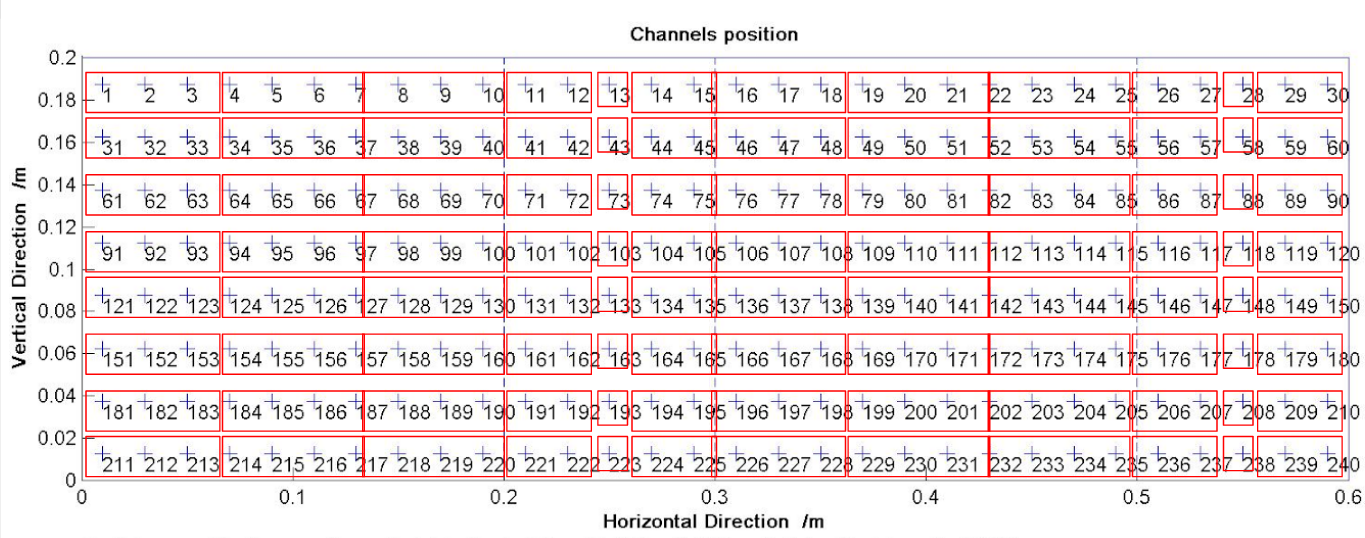
\includegraphics[width=1\linewidth]{img/tpu_windows.png}
			\label{fig:tpuwindows}
			\begin{flushleft}
				Fonte: \citeauthoronline{TPU2018} \cite{TPU2018}, adaptado pelo autor.
			\end{flushleft}
		\end{figure}
		
		
		\subsection{Simulações simplificadas}
		
		Nesta etapa do método, buscou-se simplificar o modelo de escritório desenvolvido no EnergyPlus, atentando-se às limitações relacionadas à simplificação do modelo.
		O objetivo de gerar um metamodelo por meio de redes neurais artificiais (RNA) para se obter a EHF faz com que se busque parametrizar ao máximo as simulações no EnergyPlus.
		Essa parametrização pode facilitar o desenvolvimento de amostras para a pesquisa, assim como garantir uma relação mais direta dos parâmetros de entrada com os dados de saída. 
		Dentre as simplificações consideradas, estão:
		
		\begin{itemize}
		\item cálculo do Cp através do método analítico, em vez dos valores obtidos por medições em túnel de vento pela TPU;
		\item representação dos materiais da envoltória através de duas camadas: uma camada representando a capacidade térmica, e uma camada para regular a transmitância;  %(concreto)  (objeto Material:NoMass)
		\item modelagem da zona que representa apenas um escritório, sem modelar as demais zonas térmicas da edificação. Para isso, são definidas as condições de contorno relacionadas às faces da zona correspondentes a paredes adjacentes à edificação;
		\item definição de um coeficiente de infiltração relacionado à infiltração de ar pela porta, e do valor do Cp relacionado a essa porta, que no modelo de uma zona está voltada para o ambiente externo, e não para a circulação.
		\end{itemize}
		
		O impacto nos resultados das simulações foram verificados para cada uma das simplificações mencionadas. Desta forma foi definida a forma mais adequada de se simplificar o modelo, assim como a margem de erro que espera-se encontrar ao assumir tais simplificações.
		A seguir, cada uma dessas etapas é descrita.
		
%		Nem todos os parâmetros foram variados em todas as etapas deste processo. Optou-se por variar apenas os parâmetros que pudessem influenciar os resultados relacionados a cada análise. Quando não variados, os parâmtros tiveram seus valores fixados de acordo com a Tabela \ref{table:paramfix}.
%		
%		\begin{table}[h]
%			\centering
%			\caption{Parâmetros fixados na validação do modelo analítico para o cálculo do Cp.}
%			\label{table:paramfix}
%			\begin{tabular}{|c |c |}
%				\hline
%				\textbf{Parâmetro} & \textbf{Valor adotado} \\
%				\hline
%				Altura do pavimento & 15 m \\
%				\hline
%				Fator solar do vidro & 0,87 \\
%				\hline
%				Fator de abertura da janela & 1,0 \\
%				\hline
%				Capacidade térmica da parede & 155 kJ/m$^2$K \\
%				\hline
%				Absortância da parede & 0,5 \\
%				\hline 
%				Ângulo de sombreamento & 0 graus \\
%				\hline 
%			\end{tabular}
%			\begin{flushleft}
%				Fonte: o autor.
%			\end{flushleft}				
%		\end{table}
%		
%		
		\subsubsection{Cálculo do Cp pelo método analítico}
		
		O EnergyPlus, através do AFN, possui uma opção para calcular automaticamente os Cp's para as simulações.
		Quando essa opção é escolhida, o programa gera apenas um Cp por fachada da edificação, que podem ser obtidos por dois algorítimos diferentes: no caso de edificações altas (\textit{highrise}), utiliza-se o modelo de \citeauthoronline{Atkins} \cite{Atkins}; no caso de edificações baixas (\textit{lowrise}), utiliza-se o modelo de \citeauthoronline{SwamiChandra} \cite{SwamiChandra}.
		Enquanto que pelo método analítico os Cp's podem ser obtidos para quaisquer razões entre as dimensões das fachadas da edificação, os valores medidos em túnel de vento pela TPU são fornecidos para edificações com geometrias específicas.  % Ambas as fontes têm aplicação limitada a edificações retangulares.
		Os valores de Cp para o tipo de edificação abordada neste estudo são disponibilizados pela TPU para 25 geometrias diferentes, das quais 13 são para edificações \textit{highrise}, e 12 são para edificações \textit{lowrise}.
		
		Para verificar o quanto a fonte escolhida na definição dos Cp's influencia nos resultados das simulações, inicialmente verificou-se as diferenças entre os valores dos Cp's das medições em túnel de vento (fornecidos pela TPU), e os valores dos Cp's obtidos pelo método analítico (algorítimos do EnergyPlus), de acordo com a Equação \ref{eq:Cpdiff}.
		
		\begin{equation}
		\label{eq:Cpdiff}
		\Delta_{Cp,i,j,\alpha} = Cp_{TPU,i,j,\alpha} - Cp_{ANALITICO,i,\alpha}
		\end{equation}
		
		Onde:
		
		$\Delta_{Cp,i,j,\alpha}$ é igual à diferença entre o valor dos Cp's em um ponto $i$, de uma fachada $j$, para o ângulo do vento igual a $\alpha$;
		
		$Cp_{TPU,i,j,\alpha}$ é igual ao Cp disponibilizado pela base de dados da TPU para o ponto $i$ de uma fachada $j$, para o ângulo do vento igual a $\alpha$;
		
		$Cp_{ANALITICO,j,\alpha}$ é igual ao Cp calculado pelo método analítico para uma fachada de proporções iguais às da fachada $j$, para o ângulo do vento igual a $\alpha$.
		\\
		
%		Cada Cp médio ($Cp_{TPU,i,j}$), medido pela TPU em um ponto $j$ de uma fachada $i$, teve um Cp correspondente calculado pelo método analítico ($Cp_{ANALITICO, i}$), para a mesma fachada $i$. Essa subtração foi efetuada para os diferentes ângulos ($\alpha$) disponíveis na base da TPU.
%		As diferenças entre os valores dos Cp's foram calculadas obtendo-se o Cp pelo método analítico para cada fachada, de cada geometria disponível pela TPU, e subtraindo-se o valor do Cp calculado pelos valores disponibilizados pela base da TPU para a sua fachada correspondente (Equação \ref{eq:Cpdiff}).

		A partir dessas diferenças entre os valores de Cp ($\delta_{Cp}$), escolheu-se a geometria com a maior diferença absoluta média para se analisar a influência da diferença desses valores nos resultados das simulações no EnergyPlus.
		Para verificar o quanto a fonte utilizada na definição dos Cp's influencia nos resultados das simulações, as trocas de ar por hora (ACH) e a EHF foram comparadas entre simulações com Cp's medidos em túnel de vento pela TPU, e simulações com Cp's obtidos pelos métodos analíticos padrão do EnergyPlus.
				
%		Para cada uma dessas geometrias disponíveis, valores de Cp são disponibilizados para diversos pontos na fachada da edificação, de acordo com a Figura \ref{fig:tpupoints}.
%		
%		\begin{figure}[h]
%			\centering
%			\caption{Exemplo do posicionamento dos pontos com valores de Cp na fachada}
%			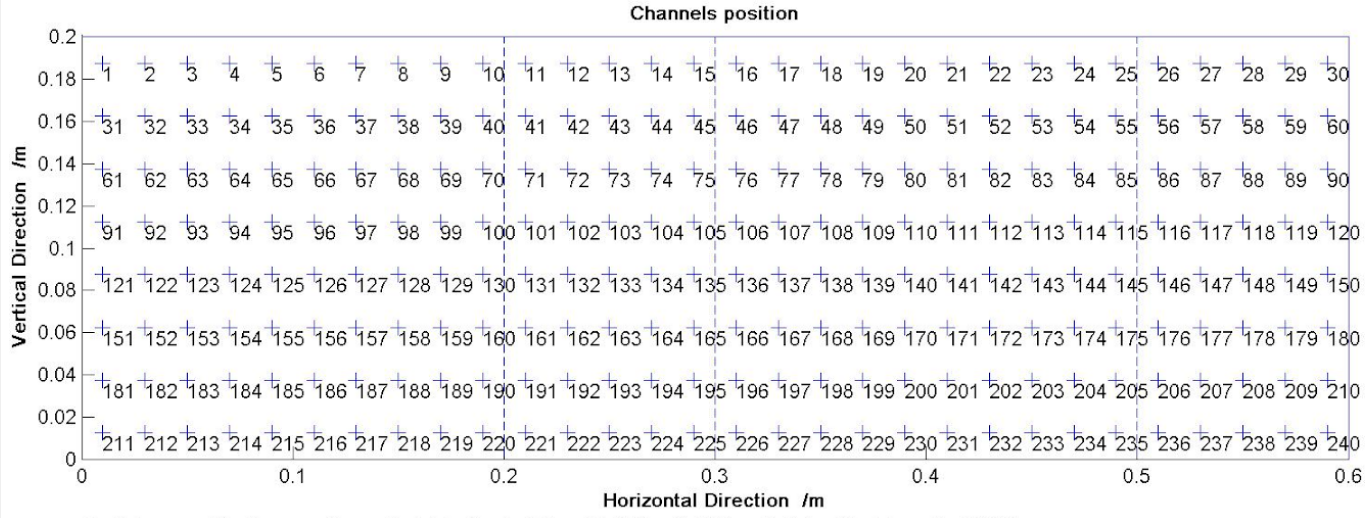
\includegraphics[width=1\linewidth]{img/tpu_points.png}
%			\label{fig:tpupoints}
%			\begin{flushleft}
%				Fonte: \citeauthoronline{TPU2018} \cite{TPU2018}, adaptado pelo autor.
%			\end{flushleft}
%		\end{figure}
		
		
		O modelo base para verificar as diferenças dos resultados utilizando-se valores de Cp com origens diferentes foi o modelo preliminar do pavimento de escritórios. Para evitar a influência do solo e da cobertura, considerou-se o pavimento intermediário. A base da TPU permite a obtenção de diferentes coeficientes de pressão para diferentes janelas, como mencionado na seção anterior. No modelo baseado no método analítico, utilizou-se um valor de Cp por fachada, devido à limitação do método. Uma amostra de 1000 casos foi gerada pelo método de amostragem do HCL. A amostra gerada teve os seguintes parâmetros variados: área da zona, altura do pavimento, azimute do eixo principal, pé-direito, PAF, fator de abertura da janela, transmitância da parede, densidade de ocupação. A razão entre largura e profundidade das zonas foi alterade para se ajustar com a geometria da edificação descrita pela base de dados da TPU utilizada como referência para a análise. Os demais parâmetros tiveram seus valores fixados de acordo com a Tabela \ref{table:paramfix}.
				
		Para cada caso da amostra, foram simulados um modelo com Cp’s baseados no método analítico, e um modelo com Cp’s baseados na base da TPU (túnel de vento).
		
		\subsection{Representação da envoltória}
		
		Para possibilitar a parametrização contínua e independente das propriedades termofísicas da envoltória, considerou-se a utilização de uma parede com propriedades equivalentes, modelada com uma camada de concreto, para representar a capacidade térmica, e uma camada modelada com o objeto Material:NoMass, para regular a transmitância.
		A validação da modelagem simplificada da parede foi feita para 3 tipos de paredes referência:
		
		\begin{itemize}
			\item parede de concreto;
			\item parede de alvenaria e reboco;
			\item parede de gesso com lã de rocha.
		\end{itemize}
		
		Como a modelagem da parede de alvenaria possui uma camada de ar no meio da parede, avaliou-se a possibilidade de considerar apenas a metade interna desta parede referência para definir a capacidade térmica da parede equivalente. Essa consideração parte do pressuposto de que a camada interna de ar faria com que a inércia térmica da metade exterior da parede não influenciasse consideravelmente a zona térmica analisada.
		
		Para validar essa simplificação, gerou-se uma amostra utilizando HCL, com 100 casos. O modelo preliminar sofreu variação dos seguintes parâmetros: área, razão entre largura e profundidade da zona, pé-direito, azimute, absortância, PAF, taxa de ocupação. Os demais parâmtros foram fixados de acordo com a Tabela \ref{table:paramfix}.
		
		Cada caso da amostra foi simulado com os três tipos de paredes diferentes, e suas paredes equivalentes. No caso da parede de alvenaria, um modelo de parede equivalente foi desenvolvido considerando-se apenas metade da parede de alvenaria.
		
		A partir dos resultados, observou-se a diferença média entre as temperaturas operativas das zonas nos modelos com as paredes referências em relação aos modelos com as respectivas paredes equivalentes. O mesmo foi feito comparando-se a EHF.
		
		\subsection{Condição de contorno das paredes adjacentes}
		
		Simular apenas uma zona, em vez de um edifício ou de um pavimento com diversas zonas, possibilita a simulação de casos diversos em menor tempo.
		
		Para modelar apenas uma zona, considerou-se as paredes correspondentes a superfícies voltadas para outros escritórios como adiabáticas. A superfície que representa a parede voltada para a circulação foi testada com duas condições de contorno: como adiabática, e como outdoors, sem incidência de vento ou sol.
		
		O modelo de referência é o modelo preliminar. Para cada caso referência, seis modelos de uma zona foram modelados, correspondendo a cada uma das zonas do modelo referência. A modelagem da ventilação natural sofre um impacto significativo quando o escritório é modelado como apenas uma zona. Esse impacto é devido à forma como a rede de fluxo de ar é montada. No caso do modelo referência, a porta é voltada para a circulação, enquanto que no caso de uma única zona, a porta desta zona é voltada para o ambiente externo. Além disso, não é possível modelar uma porta em uma parede adiabática. Para não deixar a diferença na ventilação natural influenciar as análises comparativas entre os modelos, a ventilação natural não foi modelada para esta etapa. Em vez disso, os modelos foram desenvolvidos com uma taxa de infiltração de ar constante durante a ocupação. O valor escolhido para a taxa de renovação de ar foi igual ao valor médio obtido na etapa da comparação entre os métodos de obtenção dos valores de Cp, que é igual a 30 ACH.
		
		Para validar o uso de diferentes condições de contorno, comparou-se os resultados de EHF e temperaturas operativas dos modelos de uma zona com os modelos referência. A condição de contorno com menores diferenças médias absolutas, foi escolhida para gerar o modelo simplificado.
		
		\subsection{Modelagem da ventilação natural no modelo simplificado}
		
		A modelagem da ventilação natural no modelo simplificado deve ser adaptada para se ter resultados correspondentes ao esperado em relação aos modelos referência.
		
		No AFN do EnergyPlus não é possível modelar aberturas ou infiltração de ar em superfícies adiabáticas. Para contornar esse problema, no caso de se modelar uma parede voltada para a circulação como adiabática, é possível associar a infiltração referente à porta a uma outra superfície da zona que esteja voltada para o ambiente externo. A solução para isso é modelar diretamente os objetos dos nós relacionados às aberturas dos modelos, ou seja, os coeficientes de pressão. Desta forma é possível definir valores de Cp para superfícies (seja janela ou parede) considerando-se qualquer orientação desejada, e não necessariamente a orientação definida para aquela superfície na geometria do modelo.
		
		A modelagem do fluxo de ar pelas portas dos escritórios nos modelos de uma zona foi desenvolvida com o objeto AirflowNetwork:MultiZone:Surface:Crack. O motivo para se utilizar este objeto é porque este é um objeto que pode ser associado a qualquer superfície. Portanto, o objeto crack é associado à parede externa oposta à parede que seria voltada para a circulação.
		
		Esta forma de contornar o problema da infiltração na parede adiabática impede que os valores de Cp sejam calculados automaticamente pelo EnergyPlus, portanto valores de Cp específicos são calculados para cada abertura do modelo. A fórmula utilizada para calcular os valores de Cp é a mesma do algoritmo padrão do EnergyPlus, porém a orientação da abertura é alterada conforme desejado.
		
		Além da solução descrita para atribuir adequadamente os valores de Cp às aberturas, existe outra limitação: as diferenças de pressão do ar entre as zonas dos escritórios e da circulação variam de acordo com a direção do vento, mas não de forma igual ao que se calcularia considerando-se o Cp da fachada.
		Dentro da rede de fluxo do AFN, a pressão de ar na circulação depende das trocas de ar entre todas as zonas adjacentes e das trocas de ar pelas janelas da circulação.
		Em um modelo de uma zona isso não poderia ser incluído. Para tentar contornar este problema, buscou-se uma forma de gerar um Cp equivalente para a porta no modelo de uma zona. Esse cálculo foi feito considerando-se a Equação \ref{eq:Cpeq}. A equação proposta leva em conta as resistências de todas as aberturas da edificação de referência, e calcula uma relação entre as pressões do ar externo e da circulação para cada direção de vento. Essas relações entre as pressões são adotadas então como valores de Cp, para cada orientação de vento.
		
		\begin{equation}\label{eq:Cpeq}
		C_{eq,\alpha} = \frac{P_{circ}}{P_{ext}}
		\end{equation}
		
		Onde:
		
		 $C_{eq,\alpha}$ é igual ao Cp equivalente para o ângulo $\alpha$;
		 
		 $P_{circ}$ é igual à pressão de ar na circulação;
		 
		 $P_{ext}$ é igual à pressão de ar externa. $P_{ext}$ é definida pelo EnergyPlus, baseada na velocidade do vento.
		 \\
		 
		 O valor de $P_{circ}$ é calculado baseando-se no balanço de pressões do AFN, portanto considera todo o fluxo de ar que entra e sai da zona da circulação, e a soma das diferenças de pressão é igual a zero.
		 O fluxo de ar entre as conexões consideradas como portas são calculadas como fluxo de ar por frestas, enquanto o fluxo de ar pelas conexões consideradas como janelas é calculado como uma abertura grande.
		 A pressão em cada zona, relacionada aos valores de Cp, foi calculada com um algorítmo para solucionar equações, de acordo com a Equação \ref{eq:P}:
		 
		 \begin{equation}\label{eq:P}
		 %\resizebox{\linewidth}{!}{
		 \begin{split}
		 P_{zn} = \sum_{i=1}^{N_d}{C_{porta}\times(P_{zn} - P_{conexão,i})} + \\ %
		 \sum_{j=1}^{N_w}{C_{janela}\times(P_{zn} - P_{out}\times C_{p,j})}
		 \end{split}
		 %}
		 \end{equation}
		
		Onde:
		
		$N_d$ é igual ao número de portas que se conectam à zona;
		
		$N_w$ é igual ao número de janelas que se conectam à zona;
		
		$C_{porta}$ é igual ao coeficiente relacionado à descarga de fluxo de ar pelas portas;
		
		$C_{janela}$ é igual ao coeficiente relacionado à descarga de fluxo de ar pelas janelas;
		
		$P_{conexão,i}$ é igual à pressão na zona conectada pela porta $i$;
		
		$C_{p,j}$ é o Cp na superfície da janela $j$.
		\\
		
		Devido a essas considerações, a validação foi conduzida para duas condições: considerando-se o Cp calculado diretamente pelo método analítico, e considerando-se o Cp equivalente, que leva em conta a relação entre as pressões nas zonas para cada direção de vento.
		
		Estas análises foram conduzidas considerando-se diferentes valores de coeficiente de infiltração para o objeto AirflowNetwork:MultiZone:Surface:Crack, para ajustar o valor mais adequado à taxa de infiltração que se obtém no modelo referência.
		
		%Como as taxas de infiltração são influenciadas pela temperatura do ar, as comparações com os modelos referências foram feitas considerando-se diferentes faixas de temperatura.
		
		\section{Análise de sensibilidade}
		
		Com a definição de como serão gerados os modelos simplificados, uma análise de sensibilidade será aplicada. Através da análise de sensibilidade, a influência das diferentes variáveis nos modelos serão avaliadas. Parâmetros que não sejam relevantes nos resultados de temperatura operativa e, consequentemente, fração de horas de desconforto por calor, serão fixadas.
		
		O método de \citeauthoronline{Sobol1993} \cite{Sobol1993} será utilizado para a análise de sensibilidade, pois permite a identificação de parâmetros influentes, mesmo para casos onde a relação entre as entradas e saídas dos modelos são não-monotônicas  e apresentam efeitos colineares. A amostragem para essa análise é definida pelo próprio método. A aplicação será feita através da biblioteca SALib \cite{Herman2017}, escrita na linguagem Python \cite{Python}. A partir de uma amostra com 99.978 casos, obteve-se índices de sensibilidade para análise de 1ª ordem, 2ª ordem, e total.
		
		\section{Desenvolvimento da rede neural artificial}
		
		A base de dados utilizada para o treinamento do metamodelo foi desenvolvida a partir de XXX.XXX resultados de simulações, amostrados pelo método de amostragem de Sobol. A etapa de validação foi executada com outra amostra de XX.XXX casos, amostrados pelo método do HCL. Na amostra da validação, os parâmetros não incluídos como dados de entrada para a RNA tiveram os valores fixados iguais aos da amostra utilizada para o treinamento. O motivo para se utilizar diferentes métodos de amostragem é para evitar qualquer enviesamento possivelmente relacionado ao método de amostragem.
		
		Após a etapa de validação, a amostra gerada para a AS foi utilizada para verificar o desempenho da RNA quando os valores dos parâmetros não considerados como dados de entrada da RNA variam. A escolha da amostra da etapa da AS é porque as simulações já estavam finalizadas, e os casos eram diferentes daqueles utilizados no desenvolvimento da RNA. 
		
		A forma como as variáveis descritas nos modelos simulados serão introduzidas no metamodelo a ser desenvolvido podem influenciar a precisão e a representação adequada dos fenômenos termofísicos. No processo de definição das variáveis de entrada do metamodelo, busca-se a melhor forma de descrever as diversas características das salas e do clima. Esse é um processo iterativo, no qual varia-se diferentes variáveis de entrada, utilizando-se às vezes transformações, normalizações e funções destas. É importante também observar os hiper-parâmetros (parâmetros relacionados ao processo de aprendizagem automática) escolhidos na criação da RNA. A precisão da rede pode depender do número de nós, número de camadas, assim como outros parâmetros definidos durante o processo de treinamento.
		
		Para validar a RNA, serão comparados os resultados obtidos através do metamodelo com os casos não vistos da base de dados de simulações do EnergyPlus. Como indicadores de precisão, será utilizado o erro absoluto médio e o erro absoluto do $95^{\circ}$ percentil .
		

%\bibliographystyle{lib/abntex2-num}
%\bibliographystyle{lib/abntex2-alf}
\bibliography{citacoes}
	
\end{document}